\chapter{Using RDFS-Plus in the wild}
\label{ch10}

We have seen a number of examples of the use of RDFS-Plus modeling for
merging information from multiple sources in a dynamic and flexible way.
In this chapter, we describe four  example uses of the RDFS-Plus
constructs. All of these applications of RDFS-Plus have attracted
considerable user communities in their respective fields. They
also make essential use of the constructs in RDFS-Plus, though often in
quite different ways. These are real modeling applications built by
groups who originally had no technology commitment to RDF, RDFS or OWL
(though both were conceived as RDF applications).

In the first three of these examples, a model, expressed in RDFS, is used to describe
data that is distributed on the web.  In each case, one or more applications
make use of this data to provide valuable services to some user communities.  
The fourth case is an example that uses RDFS-Plus to represent linkages between datasets
on the web. 



We already met the first application back in Section~\ref{webembed}; it is 
called \emph{Schema.org} and is used by Google, Microsoft, Yahoo and Yandex 
to describe data embedded in Web pages.  This data is used to optimize search
engine results, to provide rich snippets, and can be used for more elaborate 
applications. 

The second application is part of a major US government effort called
Data.gov (\url{http://data.gov}). Data.gov is an effort made by the US
government to publish public information. There are hundreds of
thousands of datasets in Data.gov, of which hundreds are made available
in RDF, with many more being converted all the time. Data.gov is a great
example of the data wilderness; the published data sets
come from a wide variety of source formats and collection methodologies,
resulting in idiosyncratic data representations. Data.gov shows how
technologies like RDFS and SPARQL can be useful in dealing with this
sort of data wilderness.

The third application is called \texttt{FOAF}, for ``Friend of a Friend.'' FOAF
is a project dedicated to creating and using machine-readable homepages
that describe people, the links between them, and the things they create
and do. It is based on RDF, but it originally made no commitment to RDFS
or OWL.
FOAF was originally based on RDF because of the inherently distributed
and weblike nature of the 
project requirements. As the project evolved, there was a need to
describe the relationships between various resources in a formal way;
this led it to RDFS and then on to RDFS-Plus.

The fourth example, \emph{BridgeDb}\footnote{Scientific lenses to support multiple views over linked chemistry data. Batchelor C, Brenninkmeijer C, Chichester C, Davies M, Digles D, Dunlop I, Evelo CT, Gaulton A, Goble C, Gray AJG, Groth P, Harland L, Karapetyan K, Loizou A, Overington JP, Pettifer S, Steele J, Stevens R, Tkachenko V, Waagmeester A, Williams A, Willighagen EL. In The Semantic Web – ISWC 2014, Lecture Notes in Computer Science Volume 8796, 2014, 98-113.}, is a dataset that links other data
sets for chemistry research, especially for molecular biology. 


In this chapter, we describe each of these efforts and show the use they
make of the RDFS-Plus constructs we introduced in previous chapters.

\section{Schema.org}
\label{schema.org}
While the content of Web pages, their topics, authors, context, etc. are usually easily 
understandable by humans, the data they contain are hard to extract unless they include a 
known markup. Schema.org is a joint initiative started by Google, Microsoft, Yahoo and 
Yandex to provide shared ontologies supporting the embedding of structured data in web 
pages. We saw in Section~\ref{webembed} how formats like RDFa, Microdata and JSON-LD can 
be used to embed RDF in web pages, and how such data is used to provide
advanced data application like rich snippets and enhanced search engine optimization. 
But these applications can't do their job without some sort of shared vocabulary 
for that data.  Schema.org provides a central location for this shared vocabulary. 

Millions of sites use the ontologies of Schema.org to markup their pages and improve search and user experience 
in general across applications. Although the mark up of Web pages may have been motivated by the impact it 
has on the major search engines, it also makes the embedded data available to anyone and to any Web application. 
The fact that standard syntaxes like RDFa, Microdata or JSON-LD and schemas are supported by major search 
engines has made the mark up of Web pages with structured data  widespread.  Since the W3C has standardized these
syntaxes, anyone can parse them, making this data reusable by anyone in their own application. 


The class hierarchy of Schema.org includes things that you can describe in 
your web pages. 
Commonly used classes include: Persons, Events, Organizations, Places, Creative works, non-text objects embedded in pages (Image, Video, Audio), Products and offers, Reviews and ratings, Actions (search trade, update, ...), etc.

Let's start with a simple example, of how we would mark up a product page about 
a Men's tie so that we can support a rich snippet such as the one shown in Figure~\ref{fig:ch4.RS}(a).

The namespace for Schema.org is just \texttt{https://schema.org/}. Here, we will 
use the prefix \texttt{schema:} for that. To get started, Schema.org defines a class called 
a \texttt{schema:Product}.  For any class in Schema.org, you can see the 
documentation for that class through follow-your-nose; if you type 
\texttt{http://schema.org/Product} into your web browser, you will get a page outlining
the properties that can be used with a Product and some example markup that uses them. 
For the purpose of this example, lets call this tie texttt{bnb:Buffalo}.  Then 
the simplest triples we can have for this product say that it is a product and its 
name:

\begin{lstlisting}
bnb:Buffalo  a schema:Product ;
             schema:name "Buffalo Plaid Tie - Blade and Blue" .
\end{lstlisting}

So far, we haven't provided any information beyond the title of the page.  How do we get
to the price of the item or whether it is in stock? 

These things are represented in Schema.org as an \texttt{schema:Offer}, which describes, 
for a product or service, an offer to sell it.  Hence, it is the \texttt{Offer} that has
a price, availability, etc.  The \texttt{Offer} is linked to the \texttt{Product} with a 
property called \texttt{schema:offers}:

\begin{lstlisting}
bnb:Buffalo a schema:Product ;
    schema:name "Buffalo Plaid Tie - Blade and Blue"@en ;
    schema:offers [ a schema:Offer ;
            schema:availability schema:InStock ;
            schema:price "49" ;
            schema:priceCurrency "USD"@en ] .
\end{lstlisting}

The \texttt{Offer} has all the price and availability details.  It is up to the 
application (in this case, the google search engine) to do something appropriate
with this information.  In the case of the rich snippet in Figure~\ref{fig:ch4.RS}, that
means displaying it right under the name in the search results.  The reviews and ratings 
managed in a similar way. 

The ontology of Schema.org is always growing.  In 2012, the Good Relations ontology
was integrated into Schema.org.  This integration provides more detailed descriptions of 
products, services and offerings.  We'll show an example of how Schema.org 
(using to a large extent the vocabulary from Good Relations).

\begin{example}{Plush Beauty Bar}
\label{Plushex}
Let's take an example of a day spa, which we'll call the 
\emph{Plush Beauty Bar} \footnote{This example is based on a real example from 
a day spa in West Hollywood which is no longer in operation}.   Let's see how
Plush can use Schema.org to make its customers more aware of its
offerings. 
The particular information in this example is
for educational purposes only, and does not correspond to any real
offerings by the Plush Beauty Bar. In this exposition, we will use the
namespace prefix \texttt{plush:} for all resources defined by Plush Beauty Bar.

The Plush description begins with the business entity itself, the
Plush Beauty Bar. It offers several services,
including a massage:

\begin{lstlisting}
plush:BeautyBar a schema:DaySpa ;
                schema:makesOffer plush:Offer1 ;
                schema:makesOffer plush:Offer2 ;
                schema:makesOffer plush:Offer3 ;
plush:Offer1 rdfs:label "Hour and a half massage" .
  ...
\end{lstlisting}


Plush's services come at a price, of course, and Schema.org allows Plush to
describe these.   This poses a modeling problem---if we were to
define a property called, say, \texttt{:cost}, that related an offering to a
number, we could specify the amount of the price, but in business we
need to know more about the cost than just the number, we need to know
currency as well. This means that we have to put some more information
on the cost relationship between the offering and its price. This is an
example of reification from Chapter~\ref{ch3}, and Schema.org
solves it by defining a
class called a \texttt{UnitPriceSpecification} for the full description of a
price. We'll see how Plush uses this to describe the price of their
manicure, building on the example above:

\begin{lstlisting}
plush:Offer1 a schema:Offer ;
  schema:priceSpecification plush:PriceSpec1 ;
  rdfs:label "Hour and a half massage" .
plush:PriceSpec1 a schema:UnitPriceSpecification ;
  schema:price "80.0" ;
  schema:priceCurrency "USD" .
\end{lstlisting}

This says that the massage offering has a price, which is \$80 (US).

This offering is for a particular service; we have seen the price and 
a label for the offering, 
but we haven't yet talked about the service itself.  An
offering can include several services, but in this case, the offering
includes just one--- a massage that lasts for an hour an a half.  

We'll start by describing the type of service that we'll be offering, a massage:


\begin{lstlisting}
plush:Massage a schema:Service ;
  rdfs:label "Relaxing Massage" .
\end{lstlisting}

Now, we can build that up to talk about a massage that lasts for an hour
and a half.  This is called a \texttt{schema:TypeAndQuantityNode}, and as its 
name suggests, it refers to a type and a quantity as a single node.  
So an hour and a half long  massage looks like this:

\begin{lstlisting}
plush:Massage1_5 a schema:TypeAndQuantityNode ;
    schema:amountOfThisGood "1.5" ;
    schema:unitCode unit:HR ;  
    schema:typeOfGood plush:Massage .
\end{lstlisting}

The idea of "an hour and a half" is done by specifying units (unsing \texttt{schema:unitCode} and the amount in those units (using \texttt{schema:amountOfThisGood}.  The units are specified by referring 
to another CURIE, \texttt{units:HR}.  The \texttt{units:} namespace
is short for \texttt{http://qudt.org/vocab/unit/}, referring the the Quantities, Units, Dimensions and Types ontology, which we will explore in more detail in 
Section~\ref{QUDT}. 

Finally, we can bring it all together as an offering, which includes a massage
that lasts for an hour and a half, with a price of \$80.  The data is shown in 
Turtle in Figure~\ref{fig:ch10.plushdata}, and as a graph in Figure~\ref{fig:ch10.02}.

\begin{figure}
\begin{lstlisting}
plush:BeautyBar a schema:DaySpa ;
  schema:makesOffer plush:Offer1 .
plush:Offer1 a schema:Offer ;
  schema:priceSpecification plush:PriceSpec1 ;
  schema:includesObject plush:Massage1_5 ;
  rdfs:label "Hour and a half massage" .
plush:PriceSpec1 a schema:UnitPriceSpecification ;
  schema:price "80.0" ;
  schema:priceCurrency "USD" .
plush:Massage1_5 a schema:TypeAndQuantityNode ;
  schema:amountOfThisGood "1.5" ;
  schema:unitCode unit:HR ;  
  schema:typeOfGood plush:Massage .
plush:Massage a schema:Service ;
  rdfs:label "Relaxing Massage" .
\end{lstlisting}
    \caption{full example of an offer for an hour and a half massage at the Plush Beauty Bar for \$80}
    \label{fig:ch10.plushdata}
\end{figure}

\begin{figure}
\centering
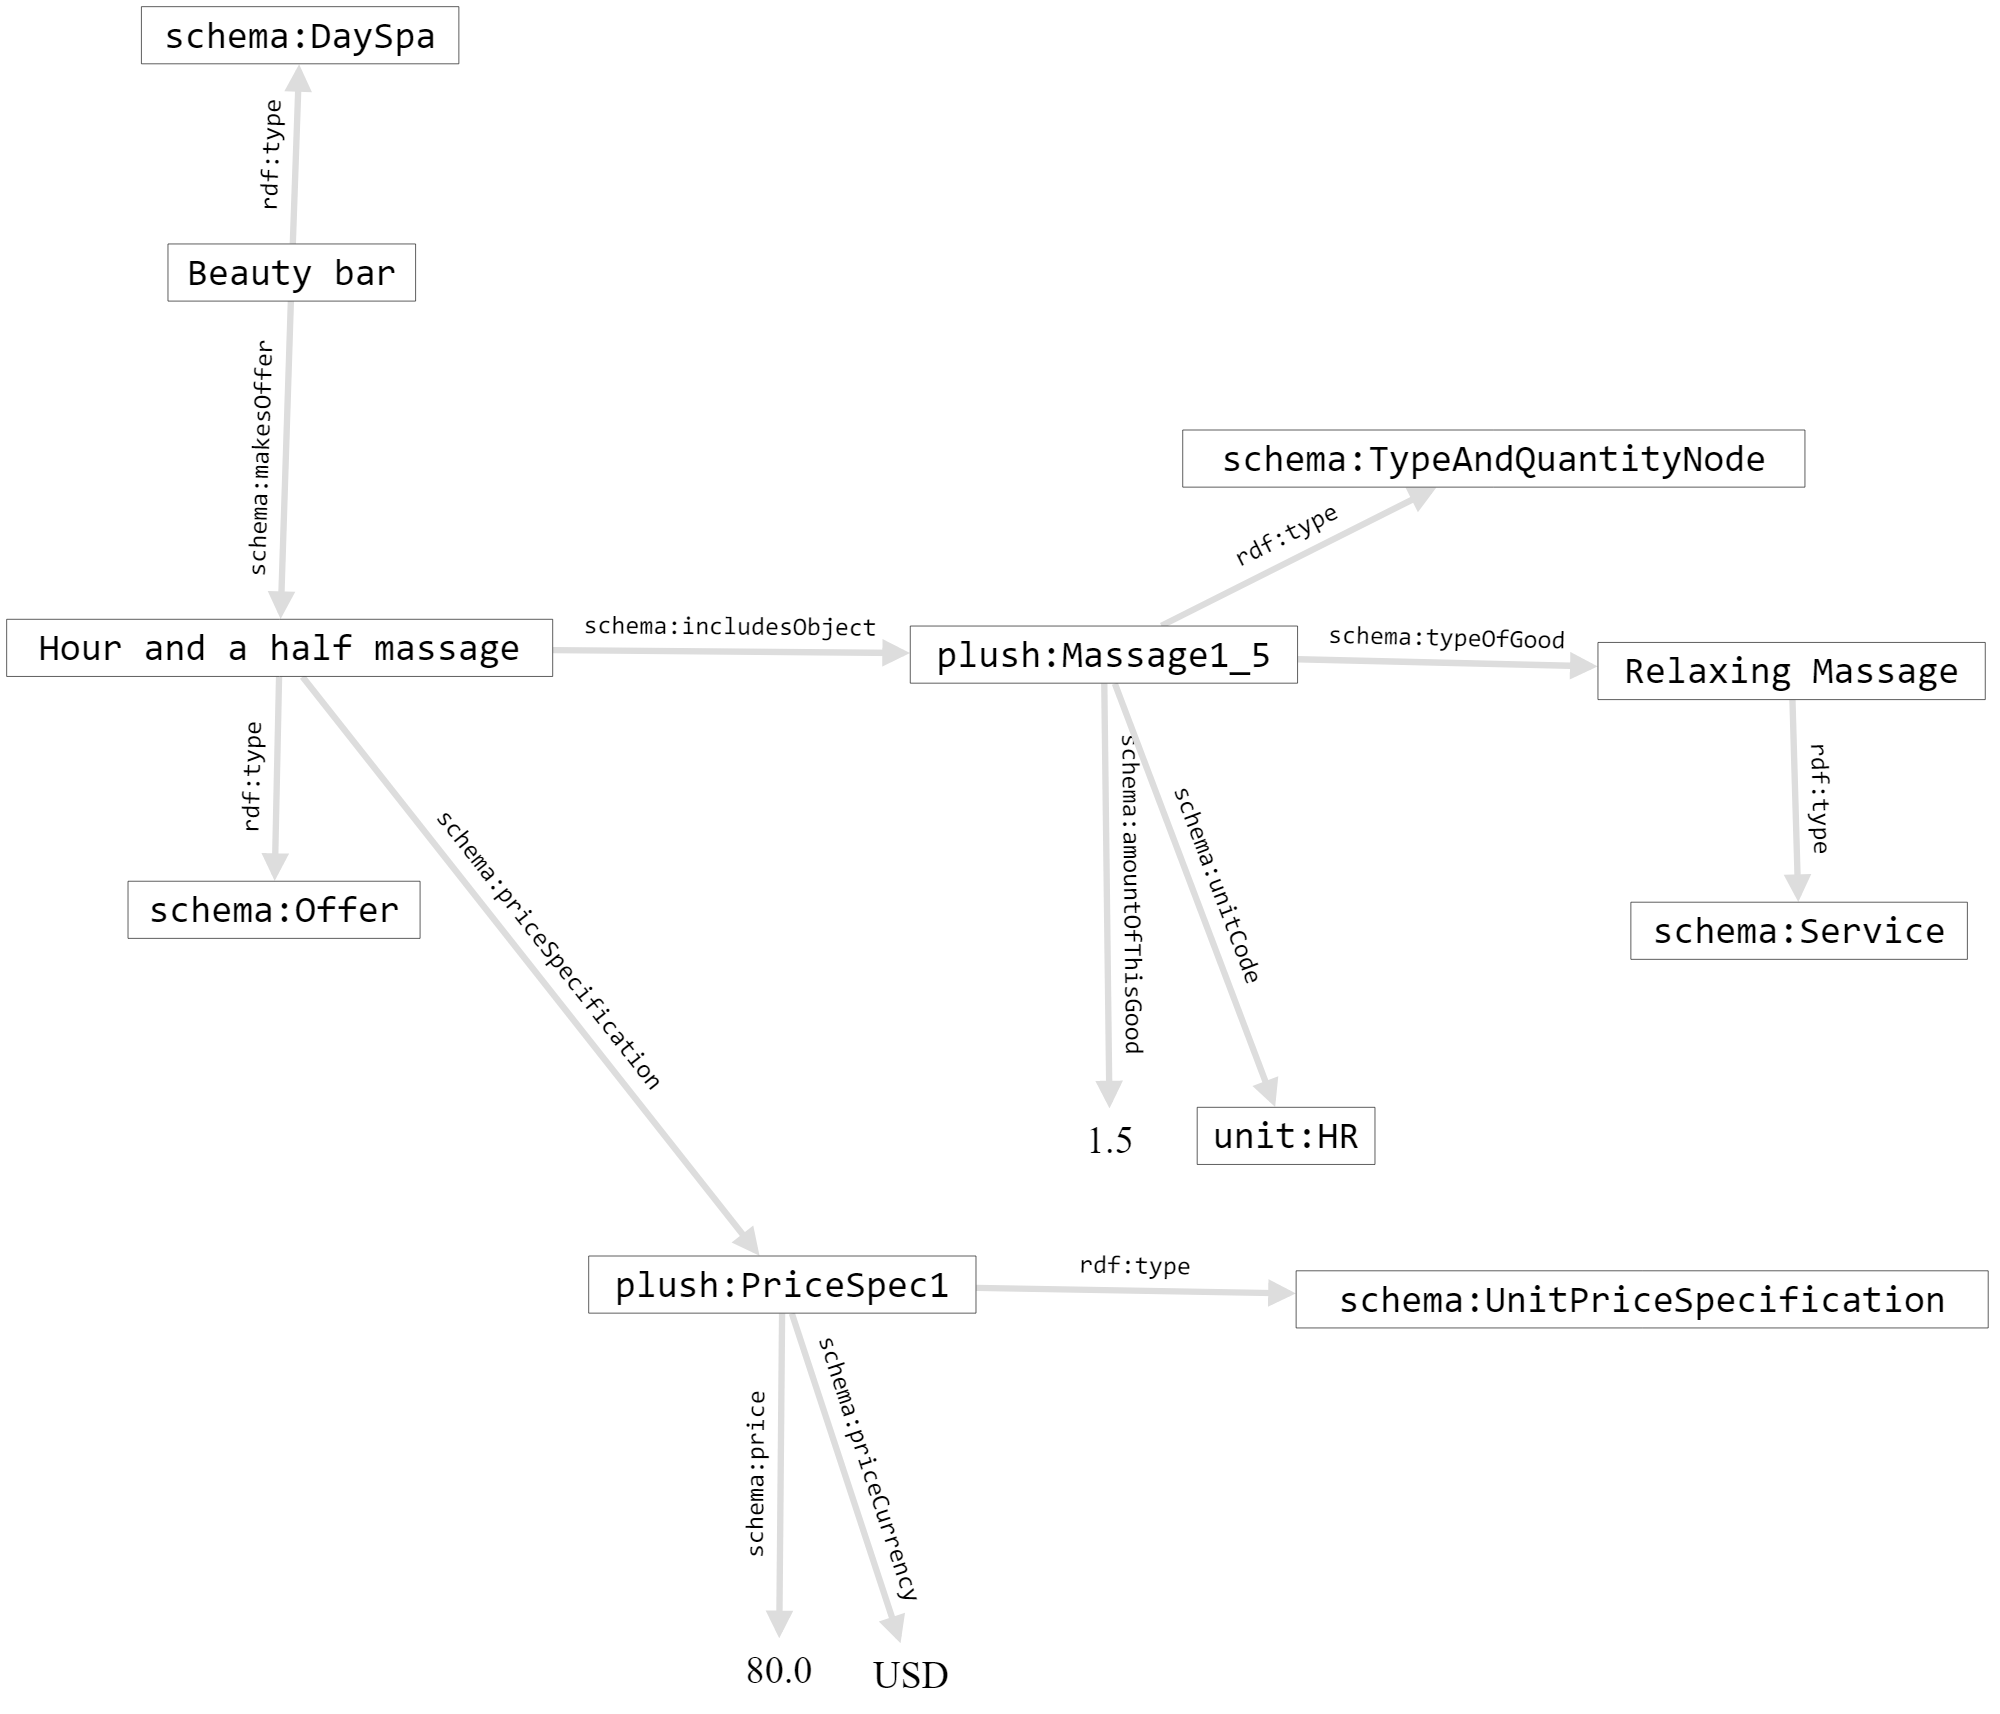
\includegraphics[width=5in]{SWWOv3/figure10-plushdata.png}
\caption{Information about Plush's massage offering, shown in graph form.}
\label{fig:ch10.02}
\end{figure}



We can query this structure of this sort to answer questions like,
``Show me the names of services that
cost less than \$100'' with SPARQL as follows:

\query{Services under \$100}
\begin{lstlisting}
SELECT ?service 
WHERE {
    plush:BeautyBar schema:makesOffer ?offer . 
    ?offer schema:priceSpecification ?amount .
    ?amount schema:priceCurrency "USD" ;
            schema:price ?price .
    ?offer schema:includesObject ?node .
    ?node schema:typeOfGood ?type .
    ?type rdfs:label ?service .
    FILTER (xsd:decimal(?price) < 100)
}
\end{lstlisting}


The results will list all the services in that price range.  The data to 
support queries of this sort is normally published on a web page, 
but Schema.org makes it possible to use it to do this sort of filtering. 
\end{example}





\subsection{Modeling in Schema.org}


At the time of this writing, Schema.org contains roughly 600 classes and nearly 
900 properties.  These numbers continue to grow, because Schema.org is being
maintained through an open community collaboration process. 

The class definitions in Schema.org are represented as \texttt{rdfs:Class}.  
For the 
example above, a few class definitions are needed, as shown in Figure~\ref{fig:ch10.s.o.def}.  These class definitions use simple concepts from RDFS, in particular, 
\texttt{rdfs:subClassOf}.  They don't give any indication about what
properties can or should be used to describe members of these classes. 


\begin{figure}
\begin{lstlisting}
schema:DaySpa
  rdf:type rdfs:Class ;
  rdfs:label "DaySpa" ;
  rdfs:subClassOf schema:HealthAndBeautyBusiness .

schema:Offer
  rdf:type rdfs:Class ;
  rdfs:label "Offer" .
  
schema:Service
  rdf:type rdfs:Class ;
  rdfs:label "Service" .
  
schema:TypeAndQuantityNode
  rdf:type rdfs:Class ;
  rdfs:label "TypeAndQuantityNode" ;
  rdfs:subClassOf schema:StructuredValue .

schema:UnitPriceSpecification
  rdf:type rdfs:Class ;
  rdfs:label "UnitPriceSpecification" ;
  rdfs:subClassOf schema:PriceSpecification .
\end{lstlisting} 

    \caption{Simple class definitions used in the Plush example. }
    \label{fig:ch10.s.o.def}
\end{figure}

In RDFS, we normally indicate the relationship between a class and the properties
we expect to use for it using \texttt{rdfs:domain}, and the expected 
type of the value for that property using \texttt{rdfs:range}.  However, as we 
saw in Section~\ref{multidomain}, the interpretation of having multiple 
\texttt{domain} (respectively \texttt{range}) declarations in RDFS is that 
we effectively express the \texttt{intersection} of the domains.  But for 
Schema.org, the desired effect is that it should be possible to express the 
\texttt{union} of multiple domains.  We saw in Section~\ref{sunion} that it is 
possible to represent something like a union in RDFS, but this involves
creating a special class for each desired union.  In the case of Schema.org, 
the requirement is simply to be able to specify a class as a domain (respectively 
range), and to have the actual domain (respectively range) be the union of all 
the classes so specified.  For this reason, Schema.org defines its own 
properties, \texttt{schema:domainIncludes} and \texttt{schema:rangeIncludes}. 
These are used just like \text{rdfs:domain} and \texttt{rdfs:range}, but 
their semantics (as suggested by the name) is that the actual domain of 
the property includes the specified class. 

As an example, in Figure~\ref{fig:ch10.plushdata} we see the use of a property 
called \texttt{schema:unitCode}.  This is how Schema.org refers to the units
for some compound value.  In our example, we specified the units for a measurement
(1.5 hours), but it is also possible to specify units for other kinds of things, 
for example, for a \texttt{schema:UnitPriceSpecification}.  This is 
handled in Schema.org with two triples about the domain, as follows:

\begin{lstlisting}
schema:unitCode
  rdf:type rdf:Property ;
  schema:domainIncludes schema:TypeAndQuantityNode ;
  schema:domainIncludes schema:UnitPriceSpecification .
\end{lstlisting}

In Schema.org, this means that the property \texttt{unitCode} can be used for any 
\texttt{TypeAndQuantityNode} and also for any \texttt{UnitPriceSpecification}.

A full analysis of the semantics of Schema.org is beyond this discussion.  The topic has been treated in 
great detail in the literature. \footnote{https://link.springer.com/chapter/10.1007/978-3-319-11964-9\_17}

\subsection{Schema.org semantics}

Schema.org made the decision to create its own modeling language, using \texttt{schema:domainIncludes} and 
\texttt{schema:rangeIncludes} instead of using the closely related constructs from RDFS of \texttt{rdfs:domain} 
and \texttt{rdfs:range}.  What are the ramifications of this decision? 

RDFS was designed with distribution of metadata in mind.  We'll illustrate this with an example.  In Finance, the 
word "principal" has two very different meanings; one refers to a debt, and is the amount of money owed.  
So when you take out a mortgage or a loan, the amount you borrow is called the "principal".  But more
generally, in a contract setting, there are some parties to the contract that are known as the "principals";
these are the main parties in the contract (while there may be many other non-principals named in the contract
as well).  There is some possibility for confusion between these terms.  

In the Semantic Web, we use URIs to denote our properties as well as anything else; suppose we have two data sets 
that use a property called \texttt{hasPrincipal}, and we want to know how each one is used.  Let's call them
\texttt{s1:hasPrincipal} and \texttt{s2:hasPrincipal}, for the usage from source 1 and 2 respectively.   Of course, 
we could have documentation in English that gives some indication of how to use each one, but that is notoriously
ambiguous and not readable by machine.  

But suppose that the data sources were to provide some machine readable modeling information about these properties, 
like this:

\begin{lstlisting}
s1:hasPrincipal rdfs:range fibo:MonetaryAmount .
s2:hasPrincipal rdfs:range fibo:ContractParty .
\end{lstlisting}

The namespace \texttt{fibo:} refers to a standard ontology about Finance, which we will describe in more detail
in Section~\ref{section:fibo}. For now, all we need to know is that FIBO provides a reference for terminology
for finance.   

Evidently, from these statements, we would like to conclude that \texttt{s1:hasPrincipal} refers to the amount of money 
in a debt, since we know that whenever that property is used in a dataset from \texttt{s1}, it will refer to a value that 
is a monetary amount.  This conclusion, that the value will \emph{always} be a member of the class \texttt{fibo:MonetaryAmount}, 
is the definition of \texttt{rdfs:range}, as given in Section~\ref{section:domainrange}.  Similar comments apply
to \texttt{s2:hasPrincipal}, by asserting these metadata statements, along with the semantics of RDFS, sources \texttt{s1}
and \texttt{s2} have communicated to people who will want to re-use their data (that is, us) how they use the 
data.  They have communicated this clearly and unambiguously.  These statements still hold in face of the Open World Assumption;
even if we learn more about \texttt{s1:hasPrincipal}, we still know that any value of this property will be a \texttt{fibo:MonetaryAmount}. 

Now suppose that \texttt{s1} and \texttt{s2} had modeled these properties using  \texttt{schema:rangeIncludes} thus:

\begin{lstlisting}
s1:hasPrincipal schema:rangeIncludes fibo:MonetaryAmount .
s2:hasPrincipal schema:rangeIncludes fibo:ContractParty .
\end{lstlisting}

Now what can we conclude?  As before, we'd like to conclude that \texttt{s1:hasPrincipal} refers to the amount of money 
in a debt (as opposed to the principal participant in a contract).  Can we infer this?  \texttt{schema:domainIncludes} tells 
us that in this data set, any time we use the property \texttt{s1:hasPrincipal}, the value for that property is either
a \texttt{fibo:MonetaryAmount} or something else, which might be specified somewhere else in their model, 
or even elsewhere on the web, if their model is also distributed.  We can't actually
conclude anything from this statement; it might be a \texttt{fibo:MonetaryAmount}, it might be a \texttt{fibo:ContractParty}, it 
might be something we haven't talked about at all, like a \texttt{schema:Offer}.  There is no conclusion we can draw at this
point. 

From a distributed metadata point of view, which is how RDFS was defined, it is clear that \texttt{rdfs:range} is more informative.
But from a master data modeling point of view, where we expect all of our metadata to be accessible in one place, \texttt{schema:rangeIncludes} 
is much more practical.  It does not require that the modelers make an unambiguous statement that will remain true even 
in the face of the open world assumption.   As a modeler, I can just gather up all the valid uses I know for a property,
and add each one as using \texttt{schema:rangeIncludes}.  As a user of metadata from \texttt{s1}, if I can know that I have seen everything 
there is to know about \texttt{s1:hasPrincipal}, then I can draw conclusions from \texttt{schema:rangeIncludes}.  In this example,
knowing that there are no more defining triples for \texttt{s1:hasPrincipal},  I can conclude that the principal 
in question is a \texttt{fibo:MonetaryAmount}

\subsection{Schema.org Summary}

Schema.org provides a way in which Web content
providers can mark up their web pages to describe business offerings.
Schema.org is based loosely on the modeling structures of RDFS, and participates
in the Semantic Web by allowing its users to make references beyond Schema.org 
(as in our example, we referred to a resource defined by QUDT). 

Schema.org's main use to date has been for Search Engine Optimization and 
rich snippets, but any application, like chatbots and personal assistants, that 
wants to make reference to data on the web, is enabled by Schema.org markup. 

Schema.org was designed with web developers in mind, so if you are maintaining 
a web site, it is straightforward to mark it up using Schema.org. 
Once you have modeled your data in Schema.org (following the examples
in this chapter), you can embed them into web pages
using any of the formats RDFa, Microdata, (Section~\ref{webembed}) or 
JSON-LD (Section~\ref{ch3.JSON}), then you can check what it means to Schema.org
by using the Google Structured Data Testing Tool \footnote{https://search.google.com/structured-data/testing-tool} or the W3C RDFa distiller \footnote{https://www.w3.org/2012/pyRdfa/} .






\section{Open Government Data}

In 2009, the US Government formalized a commitment to making public
government data open and accessible, Prior to this time, it was typical
for information to be published in the form of reports with
``infographics,'' visualizations like pie charts and times lines, which
could be printed and read by human beings, but were very difficult to
process by computer. Data.gov makes hundreds of thousands of data sets
available in a variety of machine-readable formats. The metadata for all
of these data sets, and the content for more than 500 of them, were
released as RDF in May 2010, and more are being converted now that RDF
has become one of the approved government data formats.

In the United Kingdom, a similar site called Data.gov.uk
(http://data.gov.uk) also releases many government data sets directly as
RDF. The United Kingdom has done significant work in linking these data
sets to by creating standard URIs for things such as schools and
roadways, as well as for many government agencies and functions. Many
other government organizations are also releasing data including not
just that from nations, but also from cities, states, provinces,
counties, tribal entities, etc. A number of NGOs, particularly the World
Bank and several UN units, are also releasing such data. As of the end
of 2010, the United States and the United Kingdom were the only ones
directly releasing data as RDF, although third parties in countries
around the world are now converting data from their governments to RDF
and making it available on the Web.

These open government data resources are good examples of what Tim
Berners-Lee calls ``raw'' data---machine-readable files from the
wilderness released without any specific effort to make them applicable
to a particular application. The advantage of ``raw'' data of this sort
is that it can be reused in multiple applications created by multiple
communities; but this requires some means of processing it. We will show
an example of utilizing raw open government data by examining a
particular US data set from Data.gov. This data set contains a listing
of cases filed with the FHEO (Office of Fair Housing/ Equal Opportunity)
about alleged violations of Title VIII of the Fair Housing Act. The act
protects various minorities against certain kinds of discrimination in
housing.

The FHEO data (https://catalog.data.gov/dataset/fheo-filed-cases) are available 
as a zipped Excel spreadsheet. This can be converted (as described in Challenge~\ref{chal:1}) to RDF data. 
There are over
100,000 entries that look like this:

\begin{lstlisting}
:FHEO_filed_case-0
        rdf:type  :FHEO_filed_case ;
        :case_number  "06-06-0310-8" ;
        :filing_date  "2006-01-01"^^xsd:date ;
        :number_of_filed_cases  1 ;
        :number_of_filed_cases_with_a_black_or_african_american_race_basis  1 ;
        :number_of_filed_cases_with_a_disability_basis  1 ;
        :number_of_filed_cases_with_a_familial_status_basis  1 ;
        :number_of_filed_cases_with_a_race_basis  1 ;
        :violation_county  "Lafayette" ;
        :violation_state  "Louisiana" .
\end{lstlisting}

Note that
there are several triples all with the same subject (in this case,
\texttt{:FHEO\_filed\_case-0}), and with  predicates about the basis, filing date, and
location of the discrimination complaint. The filing basis (e.g., race,
religion, color, etc.) is expressed with the value ``1'' to indicate a
factor that is a basis for the complaint; for factors that were not implicated
as a basis for the complaint, no value is recorded. This somewhat idiosyncratic
way to express the basis for the complaint is not uncommon in the data
wilderness; for example, it may have resulted from a data entry process
in which a user could put a check mark next to the basis for a report.

\begin{challenge}{How can RDFS help us organize and process FHEO data?}

\solution

A more flexible way to represent information of this sort is to define a
class of complaints based on each factor, along with a class for
complaints in general, like this:

\begin{lstlisting}
FHEO:Asian rdfs:subClassOf FHEO:Complaint .
FHEO:AsianAndWhite rdfs:subClassOf FHEO:Complaint .
FHEO:Black rdfs:subClassOf FHEO:Complaint .
FHEO:BlackAndWhite rdfs:subClassOf FHEO:Complaint .
FHEO:Color rdfs:subClassOf FHEO:Complaint .
FHEO:Disability rdfs:subClassOf FHEO:Complaint .
FHEO:FamilialStatus rdfs:subClassOf FHEO:Complaint .
FHEO:NationalOrigin rdfs:subClassOf FHEO:Complaint .
FHEO:Hispanic rdfs:subClassOf FHEO:Complaint .
FHEO:HPI rdfs:subClassOf FHEO:Complaint .
FHEO:NA rdfs:subClassOf FHEO:Complaint .
FHEO:NABlack rdfs:subClassOf FHEO:Complaint .
FHEO:NAWhite rdfs:subClassOf FHEO:Complaint .
FHEO:Other rdfs:subClassOf FHEO:Complaint .
FHEO:Race rdfs:subClassOf FHEO:Complaint .
FHEO:Religion rdfs:subClassOf FHEO:Complaint .
FHEO:Retaliation rdfs:subClassOf FHEO:Complaint .
FHEO:Sex rdfs:subClassOf FHEO:Complaint .
FHEO:White rdfs:subClassOf FHEO:Complaint .
\end{lstlisting}

We can now express the status of \texttt{:FHEO\_filed\_case-0} as a case of disability
discrimination with the single triple.

\begin{lstlisting}
:FHEO_filed_case-0 a FHEO:Disability .
\end{lstlisting}

Since \texttt{FHEO:Disability} is a subclass of \texttt{FHEO:Complaint}, we can infer from
the type propagation rule that :entry1 is also a \texttt{FHEO:Complaint}.

Building a model of this sort lets us describe our complaints in a
concise form, but it doesn't change our data---the data are still in the
form of ``1'' and ``0.'' How can we transform our data, so that all the
entries with a ``1'' for the \texttt{property:disability} become members of the
class \texttt{:Disability}, and those with a ``1'' entry for the property \texttt{:race}
become members of the class \texttt{:Race}, etc.? Each of these is easy to
accomplish with a SPARQL CONSTRUCT of the form.

\query{Classify cases by tags}
\begin{lstlisting}
CONSTRUCT {?e a :Disability}
WHERE {?e a :FHEO_filed_case ;
          :number_of_filed_cases_with_a_disability_basis "1" . }
\end{lstlisting}

We can define nineteen of these queries, one per legally identified
discrimination factor. This will construct the triple

\begin{lstlisting}
:FHEO_filed_case-0 a FHEO:Disability .
\end{lstlisting}

and others for the other classes, as desired.
\end{challenge}

SPARQL used in this way constitutes an inference method, just as RDFS
and RDFS-Plus are inference methods. In contrast to RDFS and RDFS-Plus,
SPARQL CONSTRUCT can be used to express highly customized rules about
data. In this case, we used a SPARQL CONSTRUCT to define a rule relating
the form in which we found the data, to the form we'd like it to be in.

\subsection{Describing relationships in data}

Now that we have a description of our data in classes, we can start to
describe relationships in the data in RDFS. Let's take a look at some
relationships in this data that we could express this way.

Consider the properties from the original data---things like \texttt{:race},
\texttt{:national\_origin},
\texttt{:religion}, etc. But we also have properties like \texttt{:race\_asian},
\texttt{:race\_white},
\texttt{:national\_origin\_hispanic}. One might wonder if there is some
relationship between these
values---for instance, is it true that all cases listed under
\texttt{:race\_asian} are (or should be) listed under
\texttt{:race} as well? If so, how should we represent this?

First, we can check the data to see if this is the case. Let's find out
if there is any case that lists Asian as a basis that does not also list
Race as a basis. In terms of classes, we want to find members of the
class \texttt{FHEO:Asian} that are not also members of the class \texttt{FHEO:Race}. We
can do this with an ASK query in SPARQL:

\begin{lstlisting}
ASK
{?a a FHEO:Asian .
    FILTER NOT EXISTS {?a a FHEO:Race}}
\end{lstlisting}

When we evaluate this query over the RDF version of this data set, we
get the answer \textit{false}; that is, every case of Asian bias is also a case
of racial bias. We can express a relationship like this in RDFS (thereby
expressing our opinion that this holds not just for the data we have
observed, but for all data yet to come) with a single triple in RDFS:

\begin{lstlisting}
FHEO:Asian rdfs:subClassOf FHEO:Race .
\end{lstlisting}

Similar comments apply to many of the relationships in this data. We can
express them all in, as summarized in Figure~\ref{fig:ch10.1}.

\begin{figure}
\centering
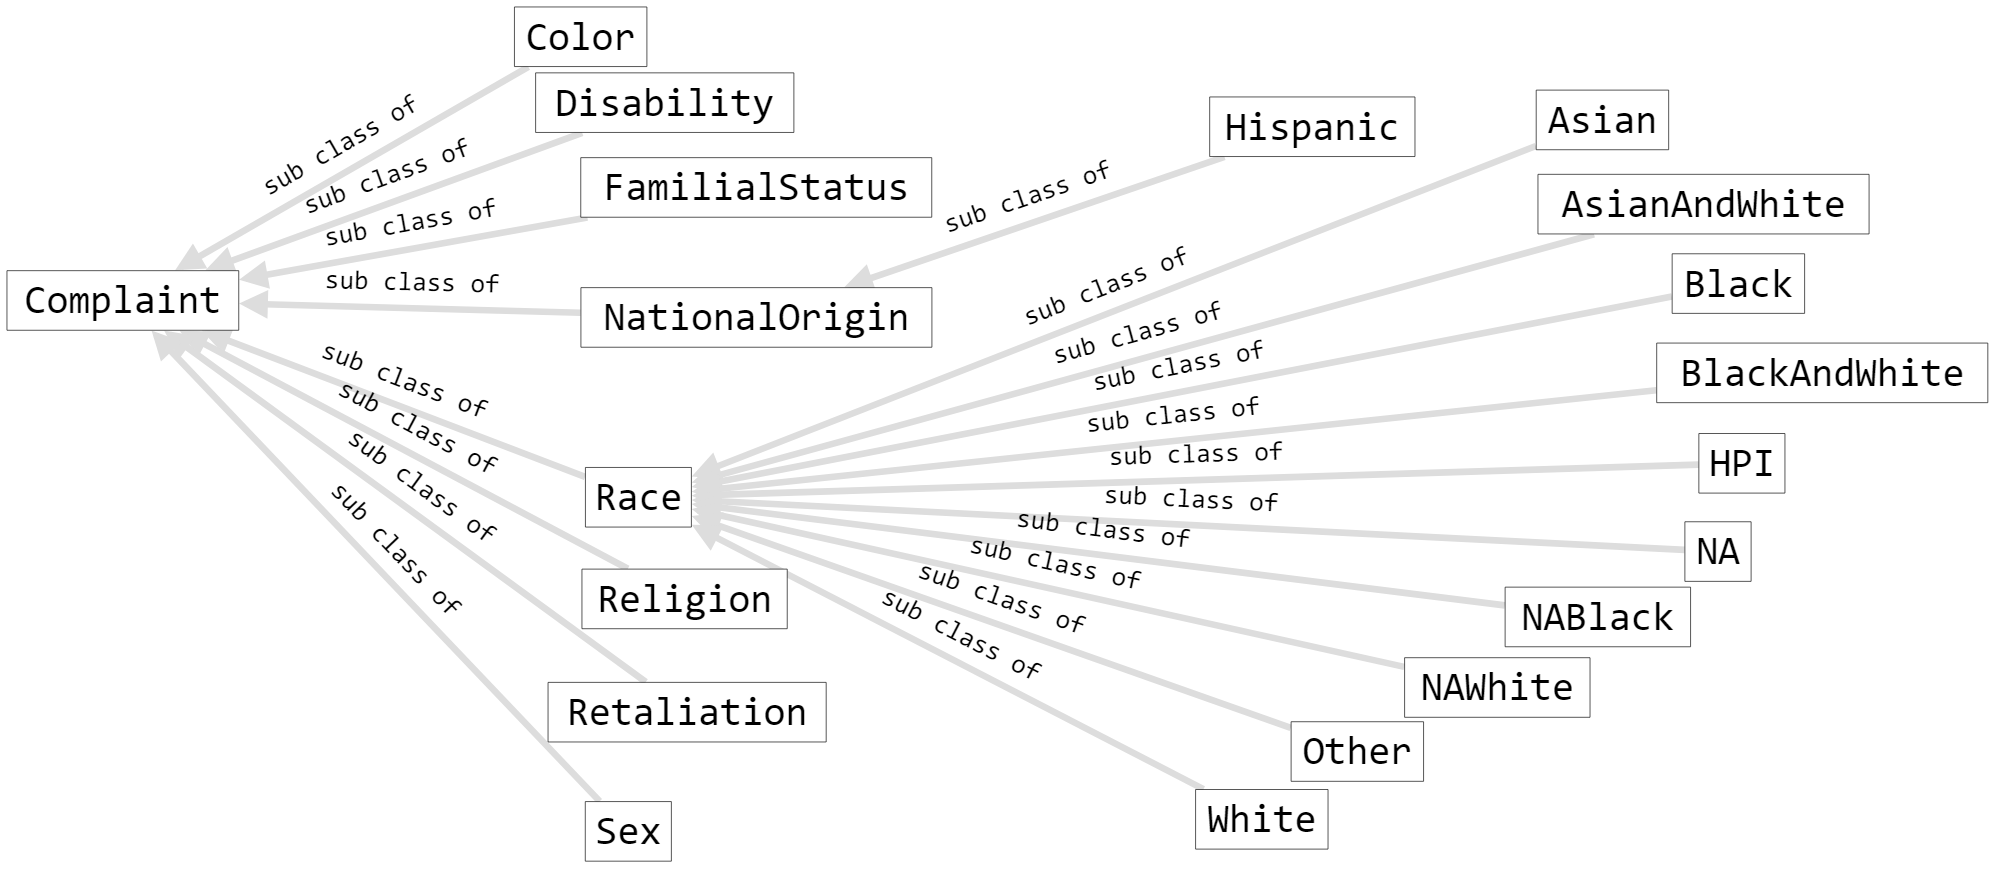
\includegraphics[width=5in]{SWWOv3/media/ch10/figure10-4.png}
\caption{Relationships between types of FHEO complaint, sorted by discrimination basis.}
\label{fig:ch10.1}
\end{figure}



We can verify this model against the current data, by using a SPARQL
query that tests every- subclass of \texttt{FHEO:Complaint}, to see whether it
has any members that are not also members of its own parent. This query
uses many of the different SPARQL constructs discussed in Chapter~\ref{ch6}:

\begin{lstlisting}
SELECT (COUNT (?suball) AS ?total) 
       (COUNT (?subonly) AS ?mismatch) ?class ?parent
WHERE {
     ?class rdfs:subClassOf+ FHEO:Complaint .
     ?class rdfs:subClassOf ?parent .
     FILTER (?parent != FHEO:Complaint)
     {
      {?suball a ?class}
     UNION
      {?subonly a ?class .
       FILTER NOT EXISTS {?subonly a ?parent}
      }
    }
}
GROUP BY ?class ?parent
\end{lstlisting}

This query finds the subclasses of \texttt{FHEO:Complaint} (leaving out the
direct subclasses), and compares each one to its own parent. The
comparison is done by finding all the complaints that are members of the
subclass, regardless of what else they might be members of (\texttt{?suball}),
and also all complaints that are members of the subclass but not members
of the parent class (\texttt{?subonly}). Finally, it counts up the number of
matches, sorted by \texttt{?class} and \texttt{?parent}. The result is given in Table~\ref{tab:ch10.1}
The results show that all the subclass relationships indeed hold in the
current data.

\subsection{Merging data with RDF and SPARQL}



\begin{table}
\caption{Results of SPARQL query, checking subClassOf relationships in
the FHEO model against current data}
\begin{tabular}{|llll|}
\hline
Total&Mismatch&Class&Parent\\
\hline
56&0&FHEO:AsianAndWhite&FHEO:Race\\
7932&0&FHEO:Hispanic&FHEO:NationalOrigin\\
483&0&FHEO:Other&FHEO:Race\\
59&0&FHEO:HPI&FHEO:Race\\
148&0&FHEO:NABlack&FHEO:Race\\
698&0&FHEO:Asian&FHEO:Race\\
2674&0&FHEO:White&FHEO:Race\\
472&0&FHEO:NA&FHEO:Race\\
89&0&FHEO:NAWhite&FHEO:Race\\
26842&0&FHEO:Black&FHEO:Race\\
1273&0&FHEO:BlackAndWhite&FHEO:Race\\

\hline
\end{tabular}
\label{tab:ch10.1}
\end{table}

This data set includes more data about each complaint than just its
type; it also includes information about the location of the complaint.
The data aren't very precise---they only show it down to the level
of one of the many hundreds of counties found in US states. But we can
take advantage of linking this information to other data to find out
where the events took place. The incident location data are in the form

\begin{lstlisting}
FHEO:filed_ca-100006
        rdf:type  FHEO:Disability ;
        FHEO:violation_county  "Franklin" ;
        FHEO:violation_state  "Ohio" .
\end{lstlisting}

Now suppose we have another data source that cross-references county names
with their location (given by latitude and longitude, by street address,
etc.). This sort of data is available from various address services
(several of which will provide it in forms that can be displayed on
Google map). To demonstrate how this works, we will use a data set
that  includes information in the form

\begin{lstlisting}
cc:Franklin_County__Ohio	
    rdfs:label "Franklin" ;
    cc:inState "Ohio" ;
	geo:lat "39.970001220703125"^^xsd:float ;
	geo:long "-83.01000213623046875"^^xsd:float .
\end{lstlisting}

We would like to be able to cross-reference our FHEO data with these
data, to find out where the alleged incidents occurred. Once again, we
can do this with SPARQL CONSTRUCT.

We can cross-refernce the violation record with the county record by 
making sure that the county names and states match for these two sources, with the following
query:

\query{Matching counties with reports}
\begin{lstlisting}
SELECT *
WHERE {
    ?complaint a ?type ;
               FHEO:violation_county ?county_name ;
               FHEO:violation_state ?state .
    ?county  rdfs:label  ?county_name ;
             cc:inState ?state .
    }
\end{lstlisting}

We can get extra information from each record.  From the county record, 
we can get the geo coordinates of the county.  From the incident record, we can get 
its type, as above:

\query{Incidents at location}
\begin{lstlisting}
SELECT ?typel ?county_name ?lat ?long 
WHERE {    
    ?type rdfs:subClassOf+ FHEO:Complaint ;
        rdfs:label ?typel .
    ?complaint a ?type ;
               col:violation_county ?county_name ;
               col:violation_state ?state .
    ?county  rdfs:label  ?county_name ;
             cc:inState ?state ;
             wgs:lat ?lat ; wgs:long ?long .
}
\end{lstlisting}

This query determines the type of the record, but only among the subtypes
of \texttt{FHEO:Complaint}, as shown in Figure~\ref{fig:ch10.1}.

This query gives us a cross-reference between complaints and the
counties they occurred in. But the reason we did this cross-reference
was so that we could get some geographical data from the second
data source, that wasn't in the first one; we get that information from
the last two triples in the graph pattern.

We can take this further, by counting the complaints per type per location, 
and filtering for only the most egregious situations, in which we had 
over 300 reports for the same location.  

\query{Counting complaint types by location}
\begin{lstlisting}
SELECT ?typel (COUNT (?complaint) AS ?severity) ?county_name ?lat ?long
WHERE {    
    ?type rdfs:subClassOf+ FHEO:Complaint ;
        rdfs:label ?typel .
    ?complaint a ?type ;
               col:violation_county ?county_name ;
               col:violation_state ?state .
    ?county  rdfs:label  ?county_name ;
             cc:inState ?state ;
             wgs:lat ?lat ; wgs:long ?long .
}
GROUP BY ?type ?typel ?county_name ?lat ?long
HAVING (?severity > 300)
\end{lstlisting}

This query combines many of the features of SPARQL from Chapter~\ref{ch6}.
Starting with the match of a complaint to a county, we also find the
type of the complaint (limited only to types that are subclasses of
\texttt{FHEO:Complaint}). Then, grouping by each type/county name/location, we count the
number of distinct complaints (as \texttt{?severity}). Finally, we sort by
severity, keeping those results having more than 300 complaints. The
results are shown in Table~\ref{tab:ch10.2}.

These results include enough information to drive an API for displaying
things on the map. If we choose an icon with a different size and
intensity for each basis and severity, then we can put these data on a
map as shown in Figure~\ref{fig:10.2}.

\begin{table}
\caption{First 10 Results of query counting number of complaints per type and county}
\label{tab:ch10.2}
\begin{tabular}{|lllll|}
\hline
Type&Severity&Countyname&Lat&Long\\
\hline
pRace&376&Cuyahoga&41.54000091552734375&-81.660003662109375\\
Black&340&Cuyahoga&41.54000091552734375&-81.660003662109375\\
Disability&468&Palm Beach&26.70999908447265625&-80.0500030517578125\\
Race&379&Jackson&39.009998321533203125&-94.339996337890625\\
NationalOrigin&353&Dallas&32.770000457763671875&-96.779998779296875\\
Black&342&Jackson&39.009998321533203125&-94.339996337890625\\
Disability&501&Bexar&29.450000762939453125&-98.51999664306640625\\
Disability&332&Jackson&39.009998321533203125&-94.339996337890625\\
Disability&358&Cuyahoga&41.54000091552734375&-81.660003662109375\\
Black&451&Harris&29.8600006103515625&-95.3899993896484375\\
\hline
\end{tabular}
\end{table}


This same method can be generalized to mash up more data sets. For
example, any data set that uses county names is amenable to this same
query. Mashing up multiple data sets is as easy as loading the new
classes for the new data sets, and letting SPARQL do the rest. This
approach is being used on US government data sets every day, providing
insight into the otherwise unmanageable data.

\subsection{data.gov Summary}

The example mashup using data.gov shown here really represents only the
tip of the iceberg of what has been done, and continues to be done, with
open government data sets. A development community has generated a large
number of applications using the RDF data from the United Kingdom, and
in the United States researchers at Rensselaer Polytechnic Institute
(RPI), have used this approach to produce a wide variety of applications
using government data, several of which are highlighted on the official
US data.gov page (See \url{http://data.gov/semantic}). The provisioning
of government data as RDF makes it easy to mix and match data sets,
producing visualizations, applications and reports that mashup
information from multiple data sets or combine government data with
other web data (Wikipedia, news articles, Google results, etc.), which
would have been significantly harder and more expensive to do with
pre-Semantic Web technologies.

\begin{figure}
\centering
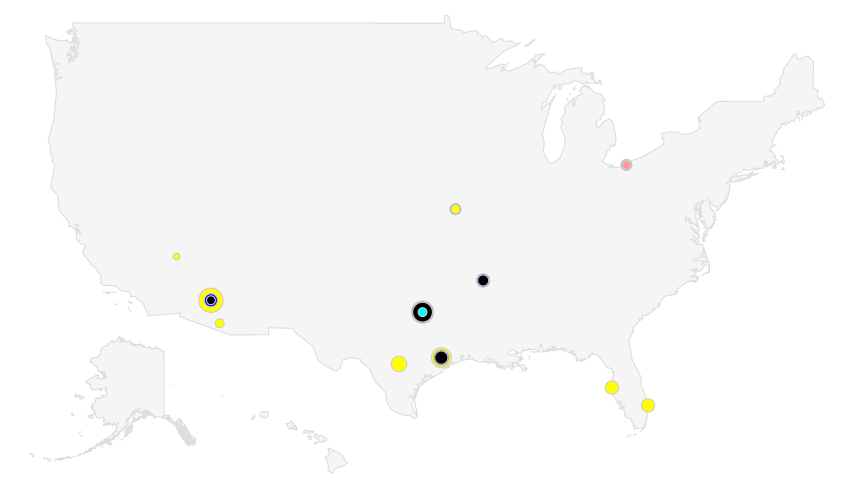
\includegraphics[width=5in]{SWWOv3/media/ch10/figure10-5.png}
\caption{Map display of the data in Table~\ref{tab:ch10.2}}
\label{fig:ch10.2}
\end{figure}


SPARQL plays a key technological role in all of these mashups. SPARQL
provides the analyst with a pattern matching tool for extracting just
the necessary information to drive a report or a display. Many of the
more advanced features of SPARQL (aggregates, filters, subqueries,
UNIONS, etc.) are put to good use in these mashup applications. (The web
site \url{http://logd.tw.rpi.edu} contains a number of demo mashups,
each linked to a page which shows the specific SPARQL queries used in
producing them.)

\section{FOAF}
\label{foaf}
FOAF (Friend of a Friend) is a format for supporting distributed
descriptions of people and their relationships. The name Friend of a
Friend is intended to evoke the fundamental relationship that holds in
social networks; you have direct knowledge of your own friends, but only
through your network can you access the friends of your friends. Though
the FOAF project dates back to early in the year 2000, and thus predated
many of the most popular social networking web sites like Instagram,
LinkedIn, and Facebook, many of the issues that FOAF was designed to
deal with were at the center of the discussion of the social network
industry ten years later and still are: privacy, ownership, and
distribution of data. FOAF began with a simple observation: If we are to
support social networks on the Web, individuals must be able to take
control of their own data, host it as they please, manage it using
whatever tools they please, but still interact with other users,
regardless of the choices these other users make. The most successful
social networking sites did not take these things into account at first;
now issues of privacy and data ownership are hot topics for any social
network. FOAF is also the basis of a number of growing ``open social''
efforts that aim to allow users to integrate their own information
across the many social- networking sites and applications available on
the Web.

FOAF works in the spirit of the AAA principle: Anyone can say Anything
about Any topic. In the case of FOAF, the topics that anyone is usually
saying things about are people. Other things that are commonly related
to what we might want to say about people, such as Organizations (that
people belong to), Projects (that people work on), Documents (that
people have created or that describe them), and Images (that depict
people), are also included in the core FOAF description. Information
about a single person is likely to be distributed across the Web and
represented in different forms. On their own web page, a person is
likely to list basic information about interests, current projects, and
some images. Further information will be available only on other pages;
a photoset taken at a party or conference could include a picture that
depicts a person who has not listed that photoset in her own web page. A
conference organizer could include information about a paper that lists
its authors, even if the authors themselves might not have listed the
paper on their own web site. A laboratory or office might have a page
that lists all of its members. FOAF leverages the distributed nature of
RDF to provide a distributed representation of this information. Social
networking sites have begun to make information available in FOAF for
web-scale distribution.

Given that there are a number of social networking web sites available
and that each one of them has a way to represent its members,
information about them, and ways in which they are connected to one
another, one could well ask why there is a need for yet another way to
describe people and their social networks. The idea of FOAF is not to
replace any of these systems but to provide a framework whereby this
information can be distributed. Furthermore, using RDF, FOAF provides a
framework that is extensible. Because Anyone can say Anything about Any
topic, FOAF allows anyone to make novel statements about people,
projects, and so on and to relate these statements to other statements
already made.

FOAF leverages the AAA principle as well as the distributed and
extensible nature of RDF in an essential way. At any point in time, FOAF
is a work in progress. There are vocabulary terms in FOAF whose
semantics are defined only by natural language descriptions in the FOAF
``standard.'' Other terms have definitions defined in RDFS-Plus that
relate them in a formal way to the rest of the description. FOAF is
designed to grow in an organic fashion, starting with a few intuitive
terms and focusing their semantics as they are used. There is no need to
commit early on to a set vocabulary, since we can use RDFS-Plus to
connect new vocabulary and old vocabulary, once we determine the desired
relationship between them.

FOAF provides a small number of classes and properties as its starting
point; these uses some of the basic constructs of RDFS-Plus to maintain
consistency and to implement FOAF policies for information merging. FOAF
is a fairly simple system for describing people, the things they create,
and the projects they participate in. It is primarily organized around
three classes: \texttt{foaf:Person}, \texttt{foaf:Group}, and \texttt{foaf:Document}.

\subsection{People and agents}

Although FOAF is primarily about people, some of the things we want to
say about people are true of other things as well: groups, companies,
and so forth. So a \texttt{foaf:Person} is defined as part of a compact hierarchy
under the general grouping of \texttt{foaf:Agent}:

\begin{lstlisting}
foaf:Person rdfs:subClassOf foaf:Agent.
foaf:Group rdfs:subClassOf foaf:Agent.
foaf:Organization rdfs:subClassOf foaf:Agent.
\end{lstlisting}

Many things we might say about a \texttt{foaf:Person} can hold for any
\texttt{foaf:Agent}. In fact, FOAF is quite liberal in this regard; most of the
properties we describe here for people hold for agents in general.
Details of exactly which properties are used for which classes are
available in the FOAF Vocabulary Specification at
\url{http://xmlns.com/foaf/0.1/}.

\subsection{Names in FOAF}

Probably the most essential thing we know about a person is that
person's name. FOAF provides a number of vocabulary terms to describe
the name of a person. Even something as simple as a person's name can be
quite complex. FOAF begins with a simple notion of name, which it
sensibly calls \texttt{foaf:name}.

\begin{lstlisting}
foaf:name rdfs:domain owl:Thing.
foaf:name rdfs:subPropertyOf rdfs:label.
\end{lstlisting}

That is, anything in the world can have a name (including a
\texttt{foaf:Person}), and that name is also used as the printable label for that
thing. For a \texttt{foaf:Person}, the name is typically the full name of the
person, like ``William Shakespeare'' or ``Anne Hathaway.''

Although the full name of a person is quite useful, parts of a person's
name are needed in some circumstances. \texttt{foaf:firstName}, \texttt{foaf:givenname},
\texttt{foaf:family\_name}, and \texttt{foaf:surname} are four properties relating to
names of people that are defined in FOAF. Each of
them has an intuitive meaning, but there are no formal semantics; the
meaning is given only in prose descriptions and by evolving conventions
of use. As FOAF evolves, it will need to encompass different cultures
and their use of names. Does the given name always come first? Is a
family name always the surname? How do culture-specific names (for
example, the ``Christian name'' that is still used in some cultures)
relate to other names?

One of the advantages to basing FOAF on RDF is that it is not necessary
to resolve all of these issues to begin the project of marking up data
using the FOAF vocabulary. The strategy taken by FOAF is to begin by
annotating a person's name while providing other naming vocabulary such
as surname, firstname, givenname, and so on. Usage patterns will dictate
which of these will turn out to be useful. If it turns out that, say,
two properties are used in exactly the same way, then this observation
can be cast by describing the relationship in OWL. For example:

\begin{lstlisting}
foaf:surname owl:equivalentProperty foaf:family_name.
\end{lstlisting}

\subsection{Nicknames and online names}

Since FOAF is primarily used on the Web, it is expected that many of the
people FOAF will be used to describe will be active in various Internet
communities. For instance, it is likely that a FOAF Person will have a
screen name on some online chat service. FOAF identifies \texttt{foaf:aimChatID},
\texttt{foaf:icqChatID}, \texttt{foaf:msnChatID}, and \texttt{foaf:yahooChatID} currently. In the
spirit of extensibility of FOAF, new ID properties can be added on an
as-needed basis. Although some part of the semantics of these properties
is given by their natural language descriptions (which connect
\texttt{foaf:yahooChatID} to the chat service Yahoo!), FOAF also makes a formal
connection between these properties. In particular, all of them are
subproperties of a single property, \texttt{foaf:nick}:

\begin{lstlisting}
foaf:aimChatID rdfs:subPropertyOf foaf:nick.
foaf:icqChatID rdfs:subPropertyOf foaf:nick.
foaf:msnChatID rdfs:subPropertyOf foaf:nick.
foaf:yahooChatID rdfs:subPropertyOf foaf:nick.
foaf:jabberID rdfs:subPropertyOf foaf:nick.
\end{lstlisting}

Following the rules of \texttt{rdfs:subPropertyOf} from Chapter 6, this means
that any \texttt{foaf:Person} who is active in chat spaces is likely to have
multiple values for the property \texttt{foaf:nick}---that is, to have multiple
nicknames. They can, of course, have further nicknames as well. For
instance, when William Shakespeare became active in Internet chat rooms,
from a FOAF point of view, all those screen names are also nicknames:

\begin{lstlisting}
lit:Shakespeare foaf:aimChatID "Willie1564".
lit:Shakespeare foaf:msnChatID "TempestMan".
lit:Shakespeare foaf:nick "Willie1564".
lit:Shakespeare foaf:nick "TempestMan".
\end{lstlisting}

Of course, we can still assert a nickname for the poet and playwright,
even if he doesn't use it as a screen name anywhere:

\begin{lstlisting}
lit:Shakespeare foaf:nick "The Bard of Avon".
\end{lstlisting}

\subsection{Online persona}

The Internet provides a number of ways for a person to express himself,
and FOAF is under constant revision to provide properties to describe
these things. A person is likely to have an electronic mailbox, and FOAF
provides a property \texttt{foaf:mbox} for this purpose. Many people maintain a
number of web pages describing parts of their lives. Some have personal
homepages, some have homepages at their workplace or school, and some
may even have both. Even their workplaces can have homepages. FOAF uses
the same strategy for these properties as it does for names: It provides
a wide array of properties, defined informally (by natural language
descriptions).

\begin{itemize}
\item \texttt{foaf:homepage}---relates a person to their primary homepage. This
property applies to anything in
FOAF, not just to people.

\item \texttt{foaf:workplaceHomepage}---the homepage of the workplace of a person.
Anything can have a homepage (even an employer), but only a \texttt{foaf:Person}
can have a workplaceHomepage.

\item \texttt{foaf:workInfoHomepage}---the homepage of a person at their workplace.
Such a page is usually
hosted by a person's employer, but it is about the person's own work
there.

\item \texttt{foaf:schoolHomepage}---the homepage of the school that a \texttt{foaf:Person}
attended. As the Internet provides new means of expression, FOAF keeps
up:

\item \texttt{foaf:weblog}---the address of the weblog of a person.
\end{itemize}

All of these properties specify instances of the class
\texttt{foaf:Document}---that is, a web page is a \texttt{foaf:Document}, a weblog is a
\texttt{foaf:Document}, and so on.

\subsection{Groups of people}

One of the interesting things about people is the groups they belong to.
FOAF provides a class called \texttt{foaf:Group} to define these groups. A group
is connected to its members via a property called, appropriately enough,
\texttt{foaf:member}. A \texttt{foaf:Group} is defined quite loosely; any grouping of
people can be described this way. For instance, we could define a group
called English Monarchy as follows:

\begin{lstlisting}
:English_Monarchy
     a foaf:Group ;
     foaf:name "English Monarchy" ;
     foaf:homepage "http://www.monarchy.com/" ;
     foaf:member :William_I, :Henry_I, :Henry_II,
             :Elizabeth_I, :Elizabeth_II.
\end{lstlisting}

A group in FOAF is an individual of type \texttt{foaf:Group}. As such, there are
a number of properties that can describe it, like \texttt{foaf:name} (as we see
here). In fact, a \texttt{foaf:Group} has a lot in common with a \texttt{foaf:Person}; it
can have a chat ID, a nickname, an email box, a homepage, or even a
blog.

It is also useful to consider the members of a group as instances of a
class---that is, to relate the instance of \texttt{foaf:Group} to an \texttt{rdfs:Class}.
For this purpose, FOAF provides a link from a group to a class, called
\texttt{foaf:membershipClass}. Suppose that the membership class for
English\_Monarchy is called Monarch; this connection is expressed in
FOAF with the triple.

\begin{lstlisting}
:English_Monarchy foaf:membershipClass :Monarch.
\end{lstlisting}

The members of the group English\_Monarchy all have type \texttt{:Monarch}:

\begin{lstlisting}
:William_I a :Monarch.
:Henry_I a :Monarch.
:Henry_II a :Monarch.
:Elizabeth_I a :Monarch.
:Elizabeth_II a :Monarch.
\end{lstlisting}

Ideally, all of these triples should be maintained automatically; that
is, any individual of type \texttt{Monarch} should appear as a member of the
group \texttt{English\_Monarchy} and every member of the group \texttt{English\_Monarchy}
should have \texttt{Monarch} as a type. This stipulation is stated explicitly as
part of the FOAF description. We will see in Chapter~\ref{ch12} how to use the
capabilities of OWL to build a model from which we can infer these
triples. The distinction between the instance \texttt{English\_Monarchy} and the
class \texttt{Monarch} is a subtle one: The class \texttt{Monarch} is a type in RDFS, and
as such, it refers to schematic things about monarchs---property
domains, subclasses, and so on. \texttt{English\_Monarchy}, on the other hand,
refers to the institution of the monarchy itself, which refers to things
like this history of the monarchy, web pages and books about the
monarchy, and so on.

In our examples so far, we have kept the world of classes separate from
the world of instances. The only relationship between an instance and a
class has been the \texttt{rdf:type} property. The intuition behind
\texttt{foaf:membershipClass} is that it indicates a class, whose instances are
exactly the same as the members of the group. The expression of this
kind of relationship, in which we sometimes wish to view something as an
instance (e.g., \texttt{English\_Monarchy}, an instance of the class \texttt{foaf:Group})
and sometimes as a class (e.g., the class \texttt{Monarch}, representing all the
instances that are \texttt{foaf:member} of that group), is an example of a
practice called metamodeling. We will see more about metamodeling when
we learn about the rest of the OWL language, and we will see how we can
use metamodeling constructs in OWL to formalize the relationship between
a \texttt{foaf:Group} and its \texttt{foaf:membershipClass}.

\subsection{Things people make and do}

Interesting people create things. They write books, publish web pages,
create works of art, found companies, and start organizations. FOAF
provides two properties to relate people to their creations: \texttt{foaf:made}
and \texttt{foaf:maker}. They are inverses of one another, and they relate a
\texttt{foaf:Agent} to an \texttt{owl:Thing} as follows:

\begin{lstlisting}
foaf:made rdfs:domain foaf:Agent.
foaf:made rdfs:range owl:Thing.
foaf:maker rdfs:domain owl:Thing.
foaf:maker rdfs:range foaf:Agent.
foaf:made owl:inverseOf foaf:maker.
\end{lstlisting}

That is, anything in the describable universe is fair game for being
made by some agent. Even another agent could have a \texttt{foaf:maker}!

If a person is an author, then he is likely to have publications to his
credit. The property \texttt{foaf:publications} relates a \texttt{foaf:Person} to any
\texttt{foaf:Document} published. Interestingly, FOAF does not specify that a
person has \texttt{foaf:made} any of their \texttt{foaf:publications}. In the spirit of
the AAA principle, if we were to decide to make such a statement, we
could do so simply by saying

\begin{lstlisting}
foaf:publications rdfs:subPropertyOf foaf:made.
\end{lstlisting}

\subsection{Identity in FOAF}

The main goal of FOAF is to apply the AAA principle to describing
networks of people; anyone can contribute descriptions about anyone. But
this leads to a problem: It is easy enough for me to describe myself; I
can publish a document that says whatever I wish to make known. If
someone else wants to contribute information about me (say, for example,
that the publisher of this book wants to add the information that I am
an author), how will that person refer to me? Or if I have several
profiles on different sites that I would like to merge together, how can
I link them to describe the one thing that is ``me''? This is a key
issue in social networking today---systems like OpenID provide naming
services so that individuals can have a single identity that cuts across
various social networks.

The RDF approach to this question is quite simple; RDF uses URIs to
denote the things it describes; that means that I should have a URI that
denotes me, and anyone who wants to make a comment about me can make it
using that URI. This is a simple, elegant, and standard solution to this
problem. This is the solution that OpenID uses, and, to some extent,
every social network system uses; a user's screen name becomes a URI; no
two users on the same system are allowed to have the same name, so the
referent of a URI like
\textless{}http://www.facebook.com/\%23!/markzuckerberg\textgreater{}
is unambiguous.

But FOAF is a distributed social networking system---can we expect
people to just make up a URI to refer to themselves? As social
networking matures, this solution is becoming more and more viable; in
fact, for many applications, a Facebook identity counts as a shared
identity for many other social networks as well, making it into a sort
of naming authority for the Web (as is OpenID). But widespread as these
things are, they are still not ubiquitous---one can be a very active
Internet citizen without having a Facebook account. Certainly in the
days when FOAF was young, these naming authorities were not in
widespread use. FOAF needed a way for people to refer to one another
that would use some part of the Internet infrastructure that was already
ubiquitous and familiar. Is there any identifying marker that everyone
on the Internet already has and is already familiar with?

The clearest answer to this puzzle is email. Just about anyone who is
described on the Web in any way at all has an email address. (Even in
2010, efforts like Webfinger take the same approach---they aim to take
advantage of the ubiquity and familiarity of an email address to deal
with identity on the social web). Email works quite well as an
identification mechanism; it is quite rare that two people share the
same email address. It is so rare that for the purposes of FOAF, email
can serve as a unique identifier for people on the Web. Notice that it
isn't a problem if someone has two or more email addresses or if some
email address is valid only for a limited period of time. All FOAF
requires of the email address is that another person doesn't share it
(either simultaneously or later on).

We can express this constraint in plain language by saying simply that
two people who share the same email address are in fact not two distinct
people at all but instead are the same person. As we have already seen,
RDFS-Plus has a way to formalize this relationship. When a property
uniquely identifies an individual, we say that the property is an
\texttt{owl:InverseFunctionalProperty}. So in FOAF, we can express the central
role that \texttt{foaf:mbox} plays in identifying individuals with the single
triple.

\begin{lstlisting}
foaf:mbox rdf:type owl:InverseFunctionalProperty.
\end{lstlisting}

Once we identify \texttt{foaf:mbox} as an \texttt{owl:InverseFunctionalProperty}, we
realize that a similar statement can be made about a number of the
properties we use to describe people; it is unusual for two people to
share a yahooChatID or an aimChatID. In fact, all of the following
properties in FOAF are \texttt{owl:InverseFunctionalProperties}:

foaf:aimChatID rdf:type owl:InverseFunctionalProperty. foaf:homepage
rdf:type owl:InverseFunctionalProperty. foaf:icqChatID rdf:type
owl:InverseFunctionalProperty. foaf:jabberID rdf:type
owl:InverseFunctionalProperty. foaf:mbox rdf:type
owl:InverseFunctionalProperty. foaf:msnChatID rdf:type
owl:InverseFunctionalProperty.foaf:yahooChatID rdf:type
owl:InverseFunctionalProperty.

Using the \texttt{foaf:mbox} (and similar properties) as identifiers of
individuals solves the technical problem of identifying individuals by
some preexisting identification, but it raises another problem:
Publishing someone's email address is considered a violation of privacy,
since email addresses (and chat IDs) can be used to pester or even
attack someone by sending unwanted, offensive, or just bulky mail. So if
we want to apply the AAA principle to William Shakespeare, and we know
that he uses the email address
Shakespeare@gmail.com, we can refer
to him as ``the person with email `Shakespeare@gmail.com''' (using a
blank node, as we did for Shakespeare's inspiration):

\begin{lstlisting}
[ foaf:mbox "Shakespeare@gmail.com " ]
\end{lstlisting}

When we do this, we publish his email address in plain text for
information vandals to steal and use. This isn't a very polite thing to
do to someone we know and respect. For this reason, FOAF also offers an
obfuscated version of \texttt{foaf:mbox}, called \texttt{foaf:mbox}\_sha1sum. It indicates
the result of applying a hashing function called SHA-1 to the email
address. The SHA-1 function is publicly available but very difficult to
reverse. To get the obfuscated string---f964f2dfd4784fe9d68ada960099e0b592e16a95---we apply the algorithm to Shakespeare's email
address. Now we can refer to him using this value:

\begin{lstlisting}
[ foaf:mbox_sha1sum
  "f964f2dfd4784fe9d68ada960099e0b592e16a95" ]
\end{lstlisting}

without compromising his privacy. Unfortunately, FOAF does not provide a
standard way to obfuscate the other identifying properties such as
\texttt{foaf:aimChatID}, \texttt{foaf:yahooChatID}, and so forth, although several
proposals to update FOAF include these.

\subsection{It's not what you know, it's who you know}

The key to FOAF as a social networking system is the ability to link one
person to another. FOAF provides a single, high-level property for this
relationship, called \texttt{foaf:knows}. The idea behind \texttt{foaf:knows} is simple:
One person knows another one, who knows more people, and so on, forming
a network of people who know people. There isn't a lot of inferencing
going on with \texttt{foaf:knows}; the only triples defined for it are

\begin{lstlisting}
foaf:knows rdfs:domain foaf:Person . 
foaf:knows rdfs:range foaf:Person .
\end{lstlisting}

that is, \texttt{foaf:knows} just links one \texttt{foaf:Person} to another.

The lack of inferencing over \texttt{foaf:knows} is by design; the \texttt{foaf:knows}
design is intentionally vague, to indicate some relationship between
people. Such a relationship could be concluded informally from other
information---for instance, co-authors can usually be assumed to know
one another. And while it is usual to think that if one person knows
another that the relationship is mutual, the FOAF designers
intentionally left out the assertion of \texttt{foaf:knows} as an
\texttt{owl:SymmetricProperty}, since there might even be some disagreement about
whether one person knows another. Despite its vague definition,
\texttt{foaf:knows} provides the infrastructure for using FOAF for social
networking, as it links one person to the next and then to the next and
so on.

\section{FACEBOOK'S OPEN GRAPH PROTOCOL}

FOAF may have been around the longest, but the largest social network to
date is Facebook. Facebook began life, as other social network sites
did, as a world unto itself---things were in Facebook, or they weren't.
Facebook didn't include Web pages that were outside its own network. One
of the ways Facebook has addressed this was the 2010 adoption of the
Open Graph Protocol (OGP), which allows it to integrate with other web
sites in new ways.

The first and most obvious manifestation of the OGP is an extension of a
Facebook facility called ``like.'' Every Facebook resource has a
distinctive button on it called ``like''; when a user clicks that
button, that page goes into their profile as something they like. Their
contacts can see that they like this, and they can opt to receive any
updates about the thing they ``like.'' Facebook ``like'' is a very
simple way for a user to customize their profile to reflect their own
personality.

The problem with ``like'' was that you could only ``like'' a page on
Facebook. If you read a news story at a major newspaper or saw a concert
listing that you wanted to ``like,'' there was no way to do it. The
Facebook OGP expanded the coverage of Facebook to include pages that
weren't already part of Facebook. The OGP in effect moved Facebook one
step toward being a global linked data network. The linkages aren't
profound---just people saying that they ``like'' something---but the OGP
is an innovative move toward a linked web of data.

To make this work, Facebook had to make it easy for someone to put
information on a web page--- any web page---that would allow Facebook to
treat this page as something someone could point to (``like'') in the
Facebook network. To make this happen, they had to overcome two
obstacles: First, they needed a language in which web page authors could
describe their pages to Facebook, and they needed a way for this
information to be embedded in the web page itself. (Facebook has
produced a number of different ways of putting ``like'' buttons on
pages, not just OGP.)

\subsection{The OGP model}

The Facebook Open Graph Protocol includes a very simple model that
allows web page authors to describe the multiple things their web pages
describe, in such a way that someone could ``like'' them in Facebook.
The sorts of things that someone might want to describe include Sports,
Businesses (bars, restaurants, etc.), People (actors, musicians,
authors, etc.), Places, Products, and Web sites. A non- normative
version of the OGP model in RDFS simply lists about two dozen of these
types of things one might want to describe in OGP.

OGP also defines a number of properties that one can use to describe the
things one might like. There are properties that describe location
(either with place names, like ``Palo Alto, California,'' or with
coordinates like latitude and longitude), properties for display
purposes (like an image that depicts the thing), contact information
(e.g., phone number, email, fax number), and identifiers (e.g., UPC,
ISBN or URL). The OGP model doesn't map these properties to the classes,
e.g., to say that it is a person or a business that has a phone number,
or a book that has an ISBN number, etc. It simply provides the types
(Classes) and properties.

OGP has been criticized for being insular and uncooperative because it
did not adopt existing
standards for all these things. FOAF already has properties for
contacting and identifying people; the W3C already has a standard for
geospatial models that includes properties for latitude and longitude.
Other existing or emerging standards refer to just about any of the
types or properties used by OGP. But OGP defined brand new ones. Doesn't
this contribute to the confusion of the Web, having just one more
standard?

It should be obvious to you by now that this criticism is based on a
misunderstanding of the Semantic Web. The Non-Unique Naming Assumption
admits that in a distributed system, this sort of thing will
happen---different people will come up with new names for the same old
things. We can't try to get everyone to agree to use the same
names---there are legitimate reasons why they want their own names. In
the case of Facebook, their user tests showed that content managers were
not happy with having to remember names from multiple sources---to
remember, for instance, that it was \texttt{foaf:mbox}, but \texttt{geo:lat} and \texttt{sioc:Site}
etc.; they wanted their vocabulary all in a single namespace, so that
they just had to remember a few dozen words, and they could describe
their content.

The Semantic Web solution to this is to allow all of these models to
coexist on the Web. We can have \texttt{og:email} (where ``og:'' is the namespace
prefix for the OGP) alongside \texttt{foaf:mbox}, and \texttt{og:latitude} as well as
\texttt{geo:lat}. The Semantic Web does not require that either of these systems
prevail over the other; the two can coexist. OGP can keep its single
namespace for content managers who don't want to be bothered with
multiple names, while FOAF, the W3C, and any other organization can
maintain their own models. Since everything is an RDF resource, we can
specify how they relate using RDFS-Plus.

The OGP RDFS model expresses these relationships as follows:

\begin{lstlisting}
og:latitude rdfs:seeAlso geo:lat . og:email rdfs:seeAlso foaf:mbox .
\end{lstlisting}

We could find fault in this model's lack of specificity, using
\texttt{rdfs:seeAlso} instead of something more expressive, like
\texttt{owl:equivalentProperty} from RDFS-Plus. Using \texttt{owl:equivalentProperty}
would make it clear that anything that FOAF calls an mbox is

something that OGP would call an email, and vice versa. Using
\texttt{rdfs:seeAlso} makes no such commitment---it simply indicates a resource
in FOAF that we should look at, if we are interested in knowing more
about \texttt{og:email}. But for the purposes of linking OGP with other
ontologies, \texttt{rdfs:seeAlso} does what is needed.

\subsection{Embedding OGP in a web page}

A web page author can describe what their page is about using the simple
OGP model, but they still have to publish that information somehow. The
easiest way to do this is to embed the description right in the web page
itself. This solution lets the web page author maintain a single page on
a particular subject, putting all the necessary information into that
page.

Facebook uses a simplified version of RDFa (Section~\ref{webembed}) to 
encode OGP data in a web
page. As with the vocabulary itself, user tests showed that embedding
information in the web page had to be very simple. In particular, the
web page author shouldn't have to face a lot of decisions about how to
do it.

The solution was to put all the OGP data into HTML tags in the page
header. For example, workingontologist.org, the web page for this book,
has the following information in its header:

\begin{lstlisting}
<meta property="og:type" content="book"/>
<meta property="og:url" content="http://www.workingontologist.com/"/>
<meta property="og:image" content="http://covers.elsevier.com/165_FW/9780123735560.jpg"/>
<meta property="og:site_name" content="Working Ontologist"/>
\end{lstlisting}


This tells Facebook that this site is about a book that it is called
Working Ontologist, that it is available at the URL
\href{http://workingontologist.org/}{http://workingontologist.org/,} and
provides a link to a picture of the cover. All the words that begin with
og: in this snippet are from the OGP model, as is the type ``book''.
This provides Facebook all it needs to put a ``like'' button on the
page, so that Facebook users can follow any updates that happen. We
suggest you go to the web page right now, click on this button, and see
what happens.

\section{SUMMARY}

OGP and FOAF demonstrate how fairly simple sets of modeling constructs
can be used to create extensible, distributed information networks. They
both take advantage of the distributed nature of RDF to allow extension
to a network of information to be distributed across the Web.

FOAF takes something of an evolutionary approach to information
extension. Many concepts have a broad number of terms (like the several
variants of ``name'' that we examined). FOAF can be extended as new
features are needed. For instance, \texttt{foaf:weblog} was not as important
before blogging became fashionable, but has now surpassed the more
classical \texttt{foaf:homepage} in importance.

OGP is arguably the most successful Semantic Web model ever; less than a
year after its introduction, its use on the Web is becoming
pervasive---as of late 2010 about 10--15\% of the like buttons on the
Web used the RDFa approach. With every Yahoo! shopping page, New York
Times article, CNN news story, etc., having a ``like'' button, with at
least four triples per button, it is difficult to estimate just how many
RDF triples are generated from OGP use. Its success is certainly due in
some degree to the enormous success of Facebook itself, but it is also
due to the commitment to simplicity that the

Facebook OGP made in its design. OGP includes only a couple dozen simple
types along with about the same number of properties.

OGP is also a clear example of the principles of the Semantic Web at
work. There are already any number of models about social networking
out there---FOAF being just one example. On the Web, we can't expect
everyone to agree on any one of these. Different applications have
differing needs. Facebook identified a strong need for simplicity, so it
re-invented several notions already available in other places. But that
doesn't mean that OGP creates just another impenetrable silo of
information; even at its inception, its connection to these other
systems was built-in to its model, in a machine- readable, queryable
way. OGP, from the outset, is part of a network of descriptive metadata
for entities in social networks.


\section{BridgeDb}

As we saw in Chapter~\ref{ch9}, RDFS-Plus can be used to manage identity 
across various data sets.  We saw the use of \texttt{owl:InverseFunctionalProperty}
as a way to specify key identifiers so that we can infer sameness within a 
dataset or even across datasets.  However, such a simple structure as 
\texttt{owl:InverseFunctionalProperty} is not sufficient for most notions of identity
in the data wilderness.  We often have to rely on heuristics, novel combinations
of properties, or even machine learning techniques to determine whether two 
entities are the same or not. 


In many cases, there isn't even a clear notion of what it means to be ``the same''.  
In molecular biology, two chemicals can be similar in many ways; these similarities 
determine how they will behave in many chemical reactions.  Chemicals with identical
formulas can behave differently in certain metabolic pathways, depending on the 
structure of the molecule.  This, in turn, can result in very different behaviors
phamacologically.  A high-profile example of this is Thalidomide, which appears in 
two forms, with identical chemical formulas.  A molecule of one form is the mirror-image
of the molecule in the other form.  One of these images (called \emph{stereoisomers}) 
is therapeutic (for symptoms of morning sickness).  The other causes severe birth
defects.  From a chemistry point of view, the two are the same; from a pharmacological 
point of view, they are different.  

The determination that two chemicals are the same in some way isn't just a matter of 
matching a few fields in a data record; in some cases, it can be actually be a research
project to determine all of the forms a chemical can take.  

The Semantic Web doesn't provide any specific methods for doing this sort of research, but,
as we saw as early as Chapter~\ref{ch01}, it provides a standardized way for someone 
who has done this research to publish their results.  This is idea behind BridgeDb.

In chemistry, and specifically the parts of chemistry that underlie molecular biology, genetics
and metabolomics, there are already a large number of databases that contain information 
about chemicals, genes and metabolism.  Each of these has its own identification system,
tuned to its own needs; we will examine one of these in detail in Section~\ref{section:Bio}.  
In order to do comprehensive biological research, as is required for drug discovery and 
other biological research, information from many of these databases has to be cross-referenced
in a precise an accurate way.  The correspondences between these data sets is well-known, 
but until recently, not available in one resource.  This was the motivation for \emph{BridgeDb}. 

The core of the data behind BridgeDb are the \emph{link sets}, which provide information linking
particular entities in one database to entities in another.  The link sets are organized based on 
which original data sets they link, and what types of entities they link.  The link sets are made available 
through APIs, data downloads, and through web pages that allow users to query for matching 
entities.  There are dozens of matching relationships available for how genes, compounds, proteins and 
other entities of biological interest could match together.  Figure~\ref{Fig:ch10.3} shows a small excerpt
from the sub property try used by BridgeDb. 

\begin{figure}
    \centering
    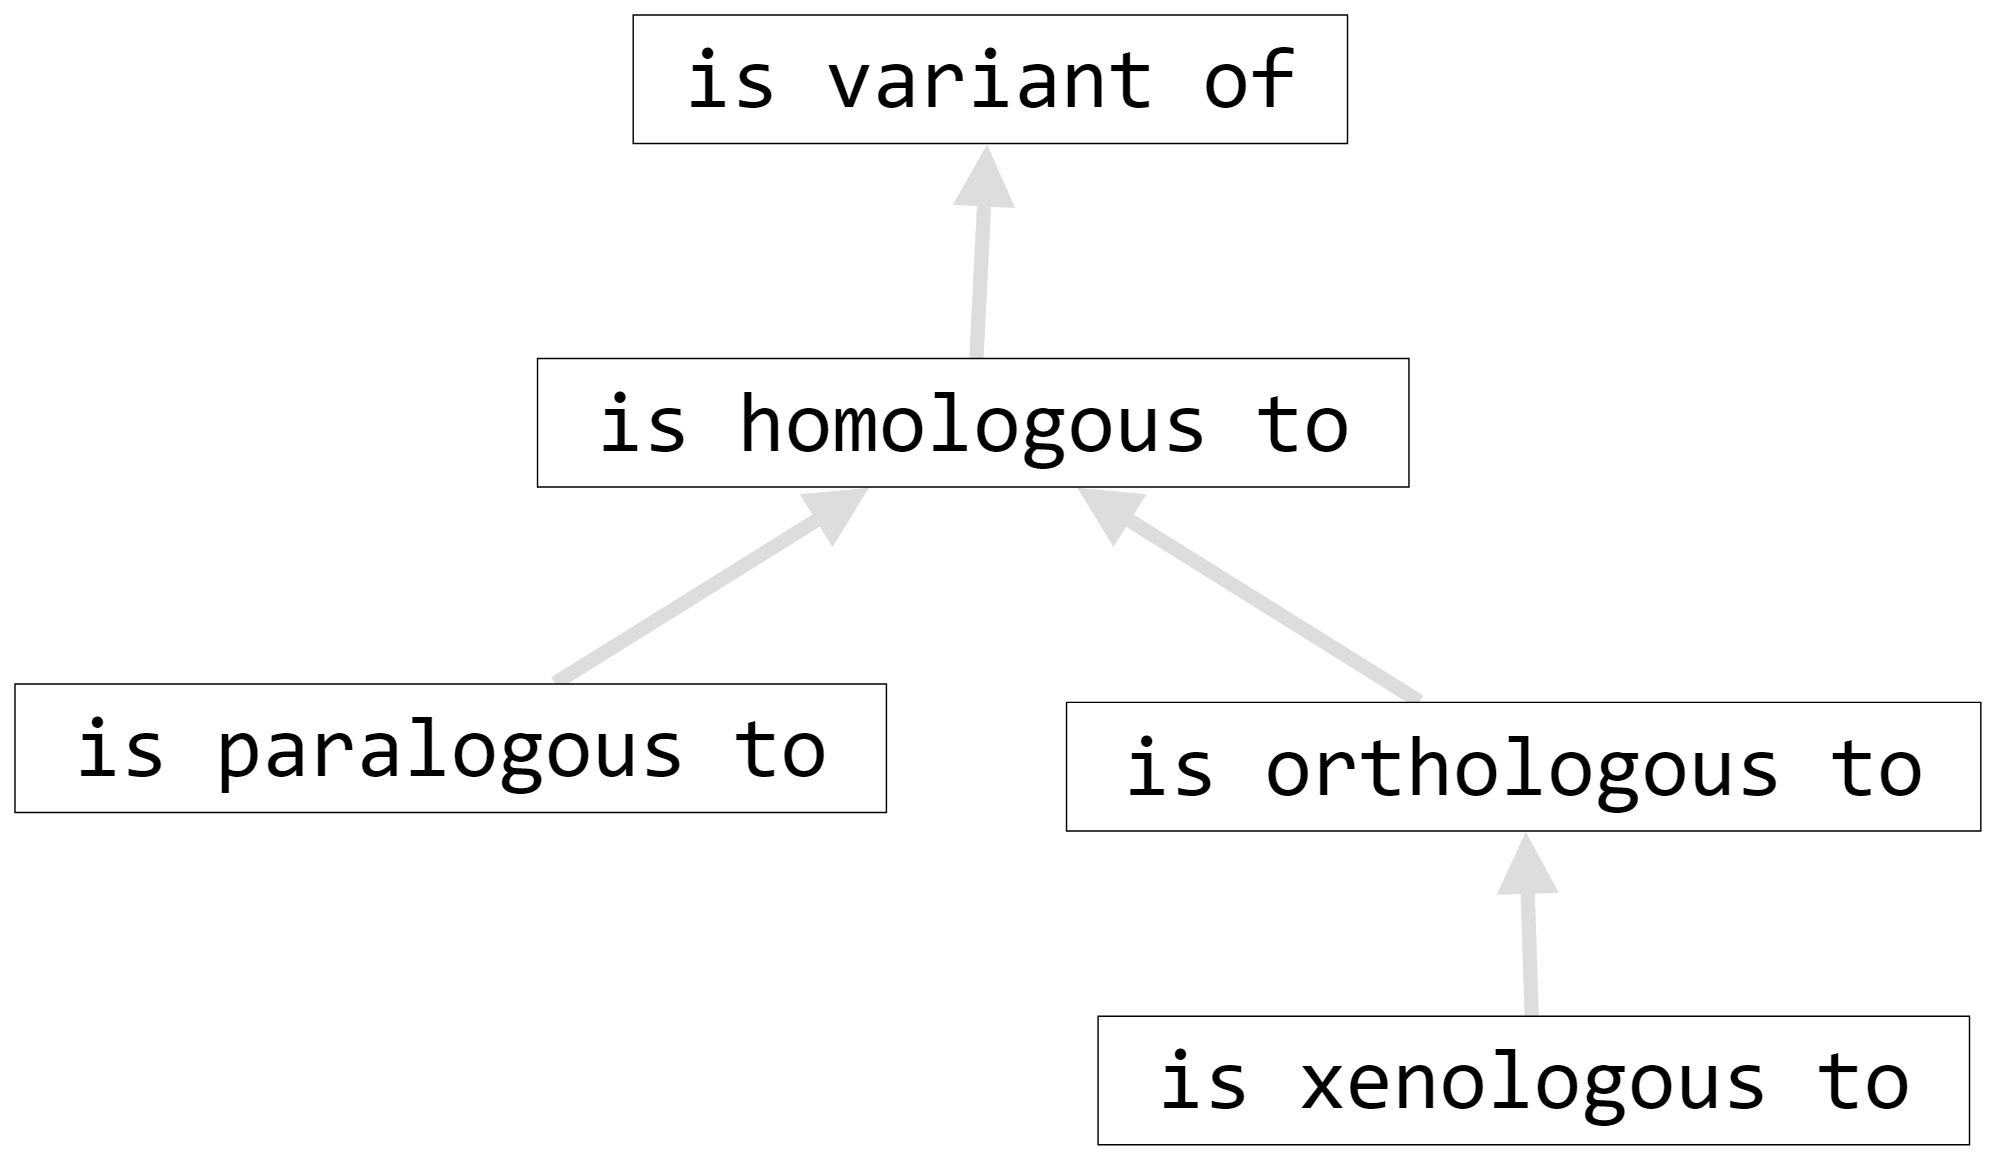
\includegraphics[width=5in]{SWWOv3/media/ch10/figure10-6.png}
    \caption{Some ways that biological entities can be related in BridgeDb}
    \label{Fig:ch10.3}
\end{figure}

BridgeDb is a fabulously useful resource, because whenever anyone wants to use one of the
source databases, there is some opportunity to use data from one of the others.  By having a 
stand-alone resource for mapping these data sets, any research that determines such 
a match is available to every user of each database.  The links between the data sets are 
as useful (or in some cases, even more so) than the datasets themselves. 




\subsection{Fundamental concepts}

The following fundamental concepts were introduced in this chapter.

Data.gov---Project to make US government spending data available in RDF.

FOAF---Namespace for a system of representation of social network
information; short for ``friend of a friend.''

Metamodeling---Generally speaking, the craft of building a model that
describes another model. A specific example is the practice of
representing a class in a model as an individual member of another
class. FOAF does this explicitly with the \texttt{foaf:membershipClass} property
that links an individual of type \texttt{foaf:Group} to the class of all members
of the group.

RDFa---a system for embedding RDF data in a web page.

OGP---the Open Graph Protocol that lets Facebook users link to pages
outside of Facebook.
